%%% Template originaly created by Karol Kozioł (mail@karol-koziol.net) and modified for ShareLaTeX use

\documentclass[a4paper,fleqn,11pt]{article}

\usepackage[T1]{fontenc}
\usepackage[utf8]{inputenc}
\usepackage{graphicx}
\usepackage{xcolor}

\usepackage{tgtermes}

\usepackage[
pdftitle={EE698G - Probabilistic Mobile Robotics Assignment}, 
pdfauthor={Satya Prakash Panuganti, 14610},
colorlinks=true,linkcolor=blue,urlcolor=blue,citecolor=blue,bookmarks=true,
bookmarksopenlevel=2]{hyperref}
\usepackage{amsmath,amssymb,amsthm,textcomp}
\usepackage{enumerate}
\usepackage{multicol}
\usepackage{tikz}

\usepackage{geometry}
\geometry{total={210mm,297mm},
left=25mm,right=25mm,%
bindingoffset=0mm, top=20mm,bottom=20mm}

\usepackage{ mathrsfs }

\linespread{1.3}

\newcommand{\linia}{\rule{\linewidth}{0.5pt}}

% custom theorems if needed
\newtheoremstyle{mytheor}
    {1ex}{1ex}{\normalfont}{0pt}{\scshape}{.}{1ex}
    {{\thmname{#1 }}{\thmnumber{#2}}{\thmnote{ (#3)}}}

\theoremstyle{mytheor}
\newtheorem{defi}{Definition}

% my own titles
\makeatletter
\renewcommand{\maketitle}{
\begin{center}
\vspace{2ex}
{\huge \textsc{\@title}}
\vspace{1ex}
\\
\linia\\
\@author \hfill \@date
\vspace{4ex}
\end{center}
}
\makeatother
%%%

% custom footers and headers
\usepackage{fancyhdr,lastpage}
\pagestyle{fancy}
\lhead{}
\chead{}
\rhead{}
\lfoot{Assignment 2}
\cfoot{}
\rfoot{Page \thepage\ /\ \pageref*{LastPage}}
\renewcommand{\headrulewidth}{0pt}
\renewcommand{\footrulewidth}{0pt}
%

%%%----------%%%----------%%%----------%%%----------%%%

\begin{document}

\title{EE698G - Probabilistic Mobile Robotics Assignment}

\author{Satya Prakash Panuganti, 14610}

\date{29 January, 2017}

\maketitle

\section{}

\begin{center}
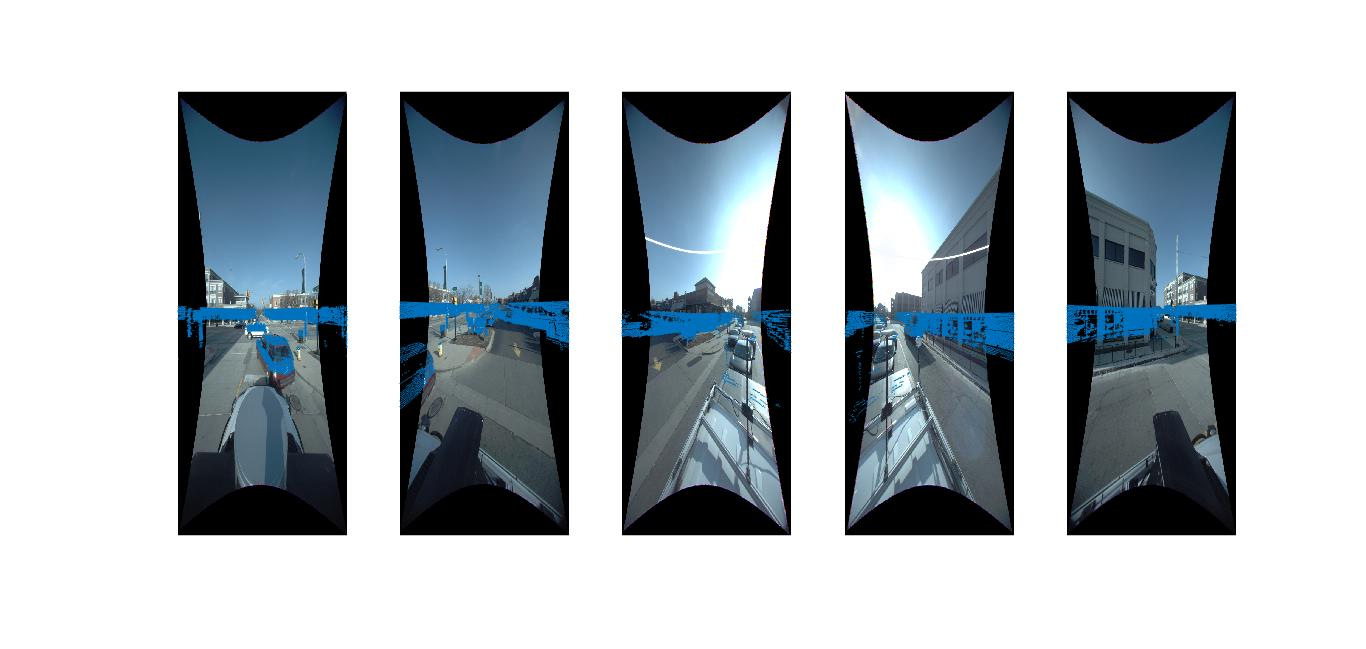
\includegraphics[scale = 0.37]{../images/q1output.jpg}
The images obatained after projecting the LIDAR points onto them.
\end{center}

\pagebreak

\section{}

\textbf{Results obtained during one run of the matlab script `question2.m' :}

\begin{center}
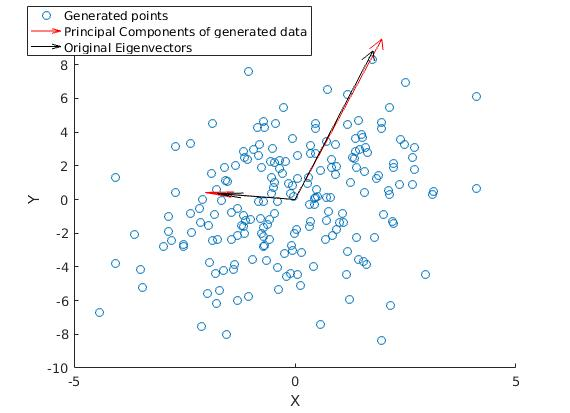
\includegraphics[scale = 0.8]{../images/q2output.jpg} \\
Visualization of gnerated datapoints, the obtained and original eigenvectors during one run of `question2.m'.
\end{center}

\begin{align*}
The\ required\ R\ matrix,\ R & = \begin{bmatrix}
									2.3077 & 1.5385 \\
									1.5385 & 9.6923
							 	  \end{bmatrix} \\
The\ covariance\ of\ generated\ datapoints,\ C & = \begin{bmatrix}
														2.6480 & 1.6817 \\
														1.6817 & 10.4508
												    \end{bmatrix} \\
The\ principal\ components\ obatined\ are\ given\ by\ : \\
\hat{\overrightarrow{x_1}} & = \begin{bmatrix}
						-2.2535 \\
						 0.4650
					 \end{bmatrix} \\
\hat{\overrightarrow{x_1}} &  = \begin{bmatrix}
									 2.1822 \\
									10.5750
					   			 \end{bmatrix}
\end{align*}
\begin{align*}
On\ rescaling\ them,\ we\ get\ : \\
\hat{\overrightarrow{x_1}} & = \begin{bmatrix}
									-4.8462 \\
									 1.0000
					  			\end{bmatrix} \\
\hat{\overrightarrow{x_1}} &  = \begin{bmatrix}
									1.0000 \\
									4.8460
					   			 \end{bmatrix}
\end{align*}
No, the obatained eigenvectors do not always match with the original eigen vectors. On running the script `question2.m' several times, it can be observed that the eigenvectors obtained change with every run of the script. \\
On running the script with a larger value of `n' (the number of points being generated), it can be seen that the obtained eigenvectors tend to be closer to the the orignal ones on increasing 'n'. This phenomenon occurs because the error in covariance of the points generated by the function 'randn' tends to go down on increasing `n', where error is the deviation of the coavariance from the identity matrix.

\section{}

\subsection*{3.a.1}
No, the euclidean co-ordinates of the points will not be normally distributed since the trasnformation from polar co-ordinates to euclidaean co-ordinates is non-linear.
\subsection*{3.a.2}

\begin{align*}
We\ have,\ X & = R\ cos\ \Theta,\ Y = R\ sin\ \Theta \\
x & = r\ cos\ \theta, y = r\ sin\ \theta \\
\implies r & = h_1(x, y) =  \sqrt{x^2 + y^2}\ \\
\&\ \theta & = h_2(x, y) = tan^{-1} \frac{y}{x} \\
The\ Jacobian,\ J & = \begin{bmatrix}
							\frac{\partial h_1}{\partial x} & 													\frac{\partial h_2}{\partial x} \\
							\frac{\partial h_1}{\partial y} & 													\frac{\partial h_2}{\partial y}
					   \end{bmatrix} \\
& = \begin{bmatrix}
		\frac{x}{\sqrt{x^2 + y^2}} & \frac{-y}{x^2 + y^2} \\
		\frac{y}{\sqrt{x^2 + y^2}} & \frac{x}{x^2 + y^2}
	\end{bmatrix} \\
Hence, |J| & = \frac{x^2 + y^2}{\sqrt{x^2 + y^2}} \\
				 & = \sqrt{x^2 + y^2} = r
\end{align*}
\begin{align*}				   
We\ know\ that\ : \\
f_{X,Y} (x, y) & = f_{\Theta,R} (\theta, r)\ |J| \\
Here,\ f_{\Theta,R} (\theta, r) & = f_{\Theta} (\theta) f_{R} (r)\ &
[\because\ R\ \&\ \Theta\ are\ independent\ variables] \\
& = \frac{1}{\sigma_\Theta \sqrt{2\pi}} e^{-\frac{(\theta - \mu_\Theta)^2}{2\sigma_\Theta^2}} \times
\frac{1}{\sigma_R \sqrt{2\pi}} e^{-\frac{(r - \mu_R)^2}{2\sigma_R^2}}  \\
& = \frac{1}{ 2\pi\sigma_\Theta \sigma_R}
e^{-[\frac{(r - \mu_R)^2}{2\sigma_R^2} + \frac{(\theta - \mu_\Theta)^2}{2\sigma_\Theta^2}]} \\
Hence,\ f_{X,Y} (x, y) & = \frac{1}{ 2\pi\sigma_\Theta \sigma_R}
e^{-[\frac{(r - \mu_R)^2}{2\sigma_R^2} + \frac{(\theta - \mu_\Theta)^2}{2\sigma_\Theta^2}]} \times (x^2 + y^2) \\
& = \frac{x^2 + y^2}{ 2\pi\sigma_\Theta \sigma_R}
e^{-[\frac{(\sqrt{x^2 + y^2} - \mu_R)^2}{2\sigma_R^2} + \frac{(tan^{-1} \frac{y}{x} - \mu_\Theta)^2}{2\sigma_\Theta^2}]} \\
Now,\ we\ have,\ \mu_\Theta & = 1, \\
				  \mu_R & = 3, \\
				  \sigma_\Theta^2 & = \frac{1}{2}
				  \implies \sigma_\Theta = \frac{1}{\sqrt{2}} \\
				  \sigma_R^2 & = 1 \implies \sigma_R = 1 \\
\therefore\ f_{X,Y} (x, y) & = \frac{x^2 + y^2}{\sqrt{2}\pi} e^{-[\frac{(\sqrt{x^2 + y^2} - 3)^2}{2} + (tan^{-1} \frac{y}{x} - 1)^2]}
\end{align*}

\subsection*{3.a.3}

\begin{align*}
Approximating\ the\ transformation\ by\ : \\
\begin{bmatrix}
	x \\
	y
\end{bmatrix} & =
\begin{bmatrix}
	\mu_R\ cos\ \mu_{\Theta} \\
	\mu_R\ sin\ \mu_{\Theta}	
\end{bmatrix} + A 
\begin{bmatrix}
	\theta - \mu_{\Theta} \\
	r - \mu_R
\end{bmatrix} \\
where,\ the\ Jacobain,\ A & = \begin{bmatrix}
						\frac{\partial r\ cos\ \theta}{\partial \theta} & 									\frac{\partial r\ cos\ \theta}{\partial r} \\
						\frac{\partial r\ sin\ \theta}{\partial \theta} & 									\frac{\partial r\ sin\ \theta}{\partial r}
					  			\end{bmatrix}_{\theta = \mu_\Theta,\
					  								 r = \mu_R} \\
 				  & = \begin{bmatrix}
				 		-r\ sin\ \theta & cos\ \theta \\
				 		 r\ cos\ \theta & sin\ \theta
				 	  \end{bmatrix}_{\theta = \mu_\Theta,\ r = \mu_R} \\
				  & = \begin{bmatrix}
						-\mu_R sin\ \mu_\Theta & cos\ \mu_\Theta \\
						 \mu_R cos\ \mu_\Theta & sin\ \mu_\Theta \\
					  \end{bmatrix} \\
Hence,\ the\ covariance\ matrix,\ \Sigma_{X,Y} & = A \Sigma_{\Theta,R} A^T \\
& = \begin{bmatrix}
		-\mu_R sin\ \mu_\Theta & cos\ \mu_\Theta \\
		 \mu_R cos\ \mu_\Theta & sin\ \mu_\Theta \\
    \end{bmatrix}
    \begin{bmatrix}
	   \sigma_\Theta^2 & 0 \\
	   0			   & \sigma_R^2
    \end{bmatrix}
    \begin{bmatrix}
		-\mu_R sin\ \mu_\Theta & \mu_R cos\ \mu_\Theta \\
		 cos\ \mu_\Theta	    & sin\ \mu_\Theta \\
    \end{bmatrix} \\
& = \begin{bmatrix}
		-2.5244 & 0.5403 \\
		 1.6209 & 0.8415
    \end{bmatrix}
    \begin{bmatrix}
	   0.5 & 0 \\
	   0   & 1
    \end{bmatrix}
    \begin{bmatrix}
		-2.5244 & 1.6209 \\
		 0.5403 & 0.8415
    \end{bmatrix} \\
& = \begin{bmatrix}
		 3.4783 & -1.5913 \\
	    -1.5913 &  2.0217
	\end{bmatrix}
\end{align*}

\subsection*{3.b.1}

\begin{center}
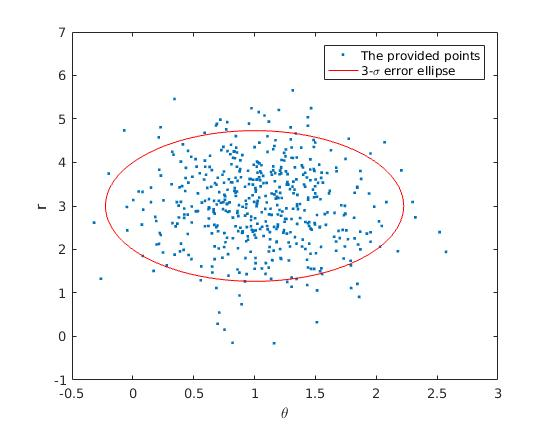
\includegraphics[scale = 0.74]{../images/q3orig.jpg} \\
The points in the file `data.mat' plotted along `$\theta$' and `r' axes.
\end{center}

\subsection*{3.b.2 \& 3.b.3}

\begin{center}
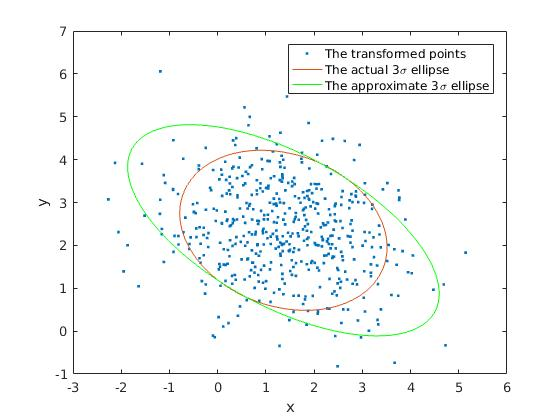
\includegraphics[scale = 0.74]{../images/q3transform.jpg} \\
The points transformed into euclidean coordinates plotted along `x' and `y' axes.
\end{center}

The sample covariance matrix of euclidean co-ordinates,
$\Sigma_{sam} = \begin{bmatrix}
					 1.5403 & -0.2846 \\
					-0.2846 &  1.1612
			    \end{bmatrix}$ \\ \\

The approximated covariance of eulcidean coordinates, 
$\Sigma_{lin} = \begin{bmatrix}
					 3.4783 & -1.5913 \\
					-1.5913 &  2.0217
			    \end{bmatrix}$
			    
\subsection*{3.b.4}

The $3\sigma$ ellipse computed by linearization appears to be skewed in a direction perpendicular to the vector connecting the origin with the mean of the transformed points. This can be explained by the fact that during linearization we expect all points with constant `r' to fall in a straight line tangent to the circle with radius `r' at the point which makes an angle `$\mu_\theta$' with the origin. However, we know that points with constant 'r' lie along a circle. Thus, during linearization we are attributing greater variance along the perpendicular than there actually is in this case.
\section{}
\begin{center}
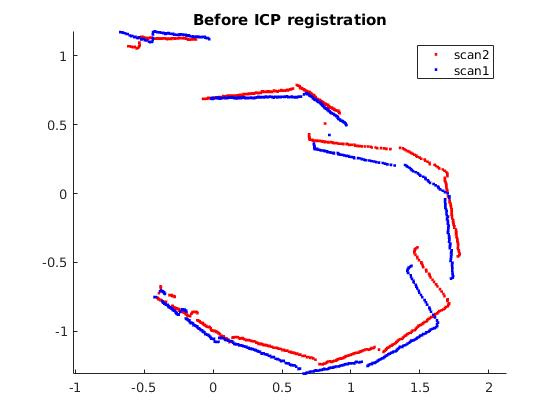
\includegraphics[scale = 0.75]{../images/q4before.jpg} \\
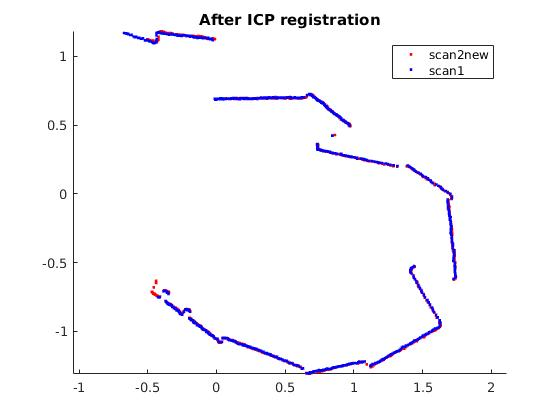
\includegraphics[scale = 0.75]{../images/q4after.jpg}
\end{center}

\section{}

Let us verify the relationship, $H_{ij} = inv\ (H_{ji})$ for a transformation in 2D. \\
\begin{figure}[!htb]
\centering
\begin{tikzpicture}[scale=0.25]

\draw[->] (5,10) -- coordinate (x axis mid) (40,10)  node[right] {$X_W$};
\draw[->] (10,5) -- coordinate (y axis mid) (10,30)  node[above] {$Y_W$}; 
%\fill[blue] (22,20) circle (8pt) node[above] {$z = a + bi$};

\draw[dashed] (30,20) -- (30,10) node[below=6pt, right=-4pt] {$t_X$};
\draw[dashed] (30,20) -- (10,20) node[left] {$t_Y$};

\draw[very thick, red] (28, 20) -- (30, 18);
\draw[very thick, red] (28, 20) -- (30.732, 20.732);
\draw[very thick, red] (30.732, 20.732) -- (30, 18);

\draw[->] (30, 20) -- (34, 24) node [anchor = south west] {$X_R$};
\draw[->] (30, 20) -- (26, 24) node [anchor = south east] {$Y_R$};

\draw[dotted] (30, 20) -- (15, 5) node[pos=0.5, blue]
								{$t_X' = -t_X\ cos\theta - t_Y\ sin\theta$};
\draw[dotted] (15, 5) -- (10, 10) node[pos=0.5, blue]
								{$t_Y' = t_X\ sin\theta - t_Y\ cos\theta$};

\draw[dotted] (30, 20) -- (34, 20);
\draw[thin] (32,20) arc(0:45:2) node[right=7pt] {$\theta$};

\draw[dotted] (32, 22) -- (29, 25) node[pos=0.5, blue] {$P_{R_Y}$};
\draw[dotted] (27, 23) -- (29, 25) node[pos=0.5, blue] {$P_{R_X}$};

\draw[dashdotted] (29, 25) -- (29, 10) node[below=6pt, left=-7pt] {$P_{W_X}$};
\draw[dashdotted] (29, 25) -- (10, 25) node[left] {$P_{W_Y}$};

\fill[black] (29, 25) circle (6pt) node[above] {$P$};

\end{tikzpicture}
\caption{\label{fig:cmpl}Robot in the world frame}
\end{figure}

Let $P_W  = \begin{bmatrix}
				P_{W_X} \\
				P_{W_Y}
		     \end{bmatrix}$
	\& $P_R  = \begin{bmatrix}
				P_{R_X} \\
				P_{R_Y}
		     \end{bmatrix}$ \\ \\

Through the use of geometry it can be shown that :
\begin{align*}
P_W & = \begin{bmatrix}
			cos \theta & -sin \theta \\
			sin \theta &  cos \theta
		 \end{bmatrix}
		 \begin{bmatrix}
		  	X_R \\
		  	Y_R
		 \end{bmatrix} +
		 \begin{bmatrix}
		  	t_X \\
		  	t_Y
		 \end{bmatrix} or \\
	& = \begin{bmatrix}
			cos \theta & -sin \theta & t_x \\
			sin \theta &  cos \theta & t_y \\
				0	   & 	   0	  &  1
		 \end{bmatrix}
		 \begin{bmatrix}
		  	X_R \\
		  	Y_R \\
		  	 1
		 \end   {bmatrix} \\
Hence,\ H_{WR} & = \begin{bmatrix}
						cos \theta & -sin \theta & t_x \\
						sin \theta &  cos \theta & t_y \\
							0	   & 	   0	  &  1
		 			\end{bmatrix} \\
Similarily,\ P_R & = \begin{bmatrix}
						 cos \theta & sin \theta \\
						-sin \theta &  cos \theta
		 		  	\end{bmatrix}
	    		  	  \begin{bmatrix}
				  		X_W \\
					  	Y_W
					  \end{bmatrix} +
					  \begin{bmatrix}
						-t_X\ cos\theta	- t_Y\ sin\theta \\
						 t_x\ sin\theta - t_Y\ cos\theta
					  \end{bmatrix} or \\
P_R & = \begin{bmatrix}
	 		 cos \theta & sin \theta & -t_X\ cos\theta	- t_Y\ sin\theta \\
	 		-sin \theta & cos \theta &  t_x\ sin\theta - t_Y\ cos\theta \\
	 			 0	    & 	   0	  &  				 1
		\end{bmatrix}
		\begin{bmatrix}
		  	X_W \\
		  	Y_W \\
		  	 1
		 \end   {bmatrix} \\
Hence,\ H_{RW} & = \begin{bmatrix}
	 			cos \theta & sin \theta & -t_X\ cos\theta	- t_Y\ sin\theta \\
	 			-sin \theta & cos \theta &  t_x\ sin\theta - t_Y\ cos\theta \\
	 			 	0	    & 	   0	  &  				 1
		 		    \end{bmatrix}
\end{align*}
\begin{align*}
Let\ us\ compute\ inv(H_{WR}) : \\
Now,\ inv(H_{WR}) & = \frac{Adjoint\ of\ H_{WR}}{det\ H_{WR}} \\
Adjoint\ of\ H_{WR} = C^T,\
						& where\ C\ is\ the\ cofactor\ matrix\ of\ H_{WR} \\
Now,\ C & = \begin{bmatrix}
	 cos\theta 						  & -sin\theta 						 & 0 \\
	 sin\theta 						  &  cos\theta 						 & 0 \\
 	-t_x\ cos\theta - t_y\ sin\theta & t_x\ sin\theta - t_y\ cos\theta & 1
		    \end{bmatrix} \\
Also,\ det\ H_{WR} & = cos^2\theta + sin^2\theta \\
		  		   & = 1 \\
\therefore\ inv(H_{WR}) & = C^T \\
& = \begin{bmatrix}
 	 cos\theta & sin\theta & -t_x\ cos\theta - t_y\ sin\theta \\
	-sin\theta & cos\theta &  t_x\ sin\theta - t_y\ cos\theta \\
		0	   &	0		&				  1			
\end{bmatrix} \\
& = H_{RW}
\end{align*}
Hence, we have verified the relationship : $H_{ij} = inv\ (H_{ji})$ for a transformation in 2D.
\end{document}